\chapter{Conception et Architecture}


\chapteropeningtext{Après avoir défini les besoins fonctionnels et les principaux cas d'utilisation de SomaScan, ce chapitre présente la conception technique de la solution. L'objectif est de décrire l'organisation générale du système, les responsabilités de chaque application, la structure interne des composants, ainsi que les choix relatifs à la base de données, aux API et à la sécurité.\par\medskip La solution repose sur une architecture composée de trois services principaux : un backend développé avec Laravel, une application mobile développée avec Flutter et une application web d'administration développée avec React. Cette séparation permet d'isoler la logique métier au niveau du backend, tout en proposant des interfaces adaptées aux différents profils d'utilisateurs.}{Architecture -- Laravel -- Flutter -- React -- API REST -- Base de données}

\section{Architecture globale du système}

SomaScan adopte une architecture client-serveur basée sur une API REST centrale. Le backend Laravel joue le rôle de coeur applicatif : il expose les endpoints, applique les règles métier, gère l'authentification, contrôle les rôles et communique avec la base de données. Les applications Flutter et React ne manipulent pas directement les données ; elles interagissent uniquement avec le backend à travers des requêtes HTTP sécurisées.

L'application mobile est destinée aux opérateurs terrain. Elle permet principalement de s'authentifier, de scanner les QR codes des camions, d'envoyer les scans au backend et de consulter l'historique récent des opérations. L'application web est destinée à l'agent logistique. Elle fournit une interface d'administration pour gérer les utilisateurs, les camions, les trajets, les rapports, les logs de scan et le tableau de bord.

La base de données MySQL ou MariaDB stocke les entités principales du système : utilisateurs, camions, trajets, logs de scan, flux de scan et jetons d'accès. Toutes les validations critiques sont effectuées côté backend afin de garantir la cohérence des données, notamment lors des opérations de scan.

La figure~\ref{fig:architecture-globale-somascan} présentera l'architecture globale de SomaScan.

\begin{figure}[H]
    \centering
    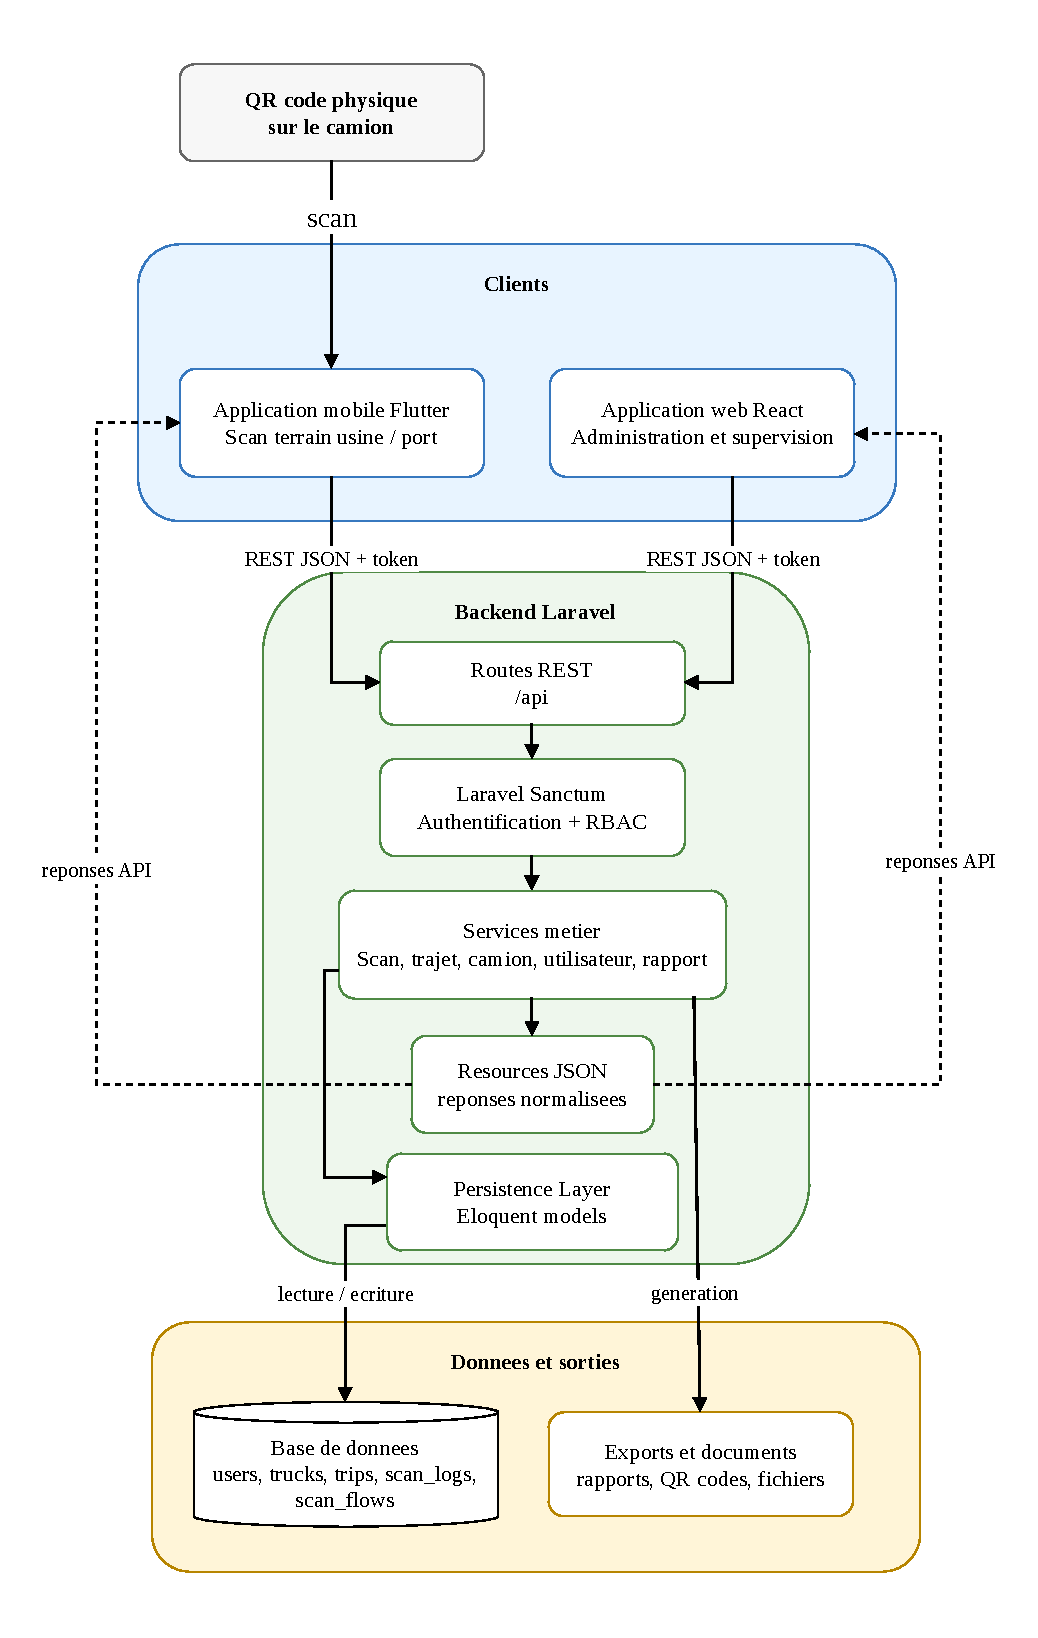
\includegraphics[width=\textwidth,height=0.88\textheight,keepaspectratio]
    {figures/architecture/architecture-global-somascan.pdf}

    \caption{Architecture globale de SomaScan}

    \label{fig:architecture-globale-somascan}
\end{figure}

\section{Architecture applicative}

\subsection{Architecture backend Laravel}

Le backend est développé avec Laravel et suit une architecture de type \textbf{Controller-Service-Model}. Ce modèle permet de séparer les responsabilités entre la gestion des requêtes HTTP, la logique métier et l'accès aux données. Les contrôleurs restent responsables de la validation des requêtes et de la construction des réponses JSON, tandis que les services regroupent les traitements métier complexes.

Les contrôleurs exposent les fonctionnalités principales : authentification, scan, gestion des camions, gestion des utilisateurs, suivi des trajets, consultation du dashboard, rapports, logs de scan et configuration du flux de scan. Les services assurent les traitements centraux, notamment la résolution des QR codes, la validation des rôles, la mise à jour des statuts de trajet, le verrouillage transactionnel, la génération des rapports et le calcul des statistiques.

Le service le plus important est le service de scan. Il orchestre le traitement d'un QR code scanné : identification du camion, vérification de son état actif, recherche du trajet courant, détermination de l'étape suivante, validation du rôle de l'opérateur, mise à jour du trajet et création du log de scan. Ce traitement est exécuté de manière transactionnelle afin d'éviter les incohérences en cas de scans simultanés.

Les modèles Eloquent représentent les principales entités métier : utilisateur, camion, trajet, log de scan et flux de scan. Les ressources Laravel permettent de formater les réponses API selon les besoins des applications clientes. Enfin, les middlewares assurent le contrôle d'accès par rôle, tandis que Laravel Sanctum fournit l'authentification par jetons.

La figure~\ref{fig:backend-laravel-architecture} présentera l'architecture interne du backend Laravel.

\begin{figure}[H]
    \centering
    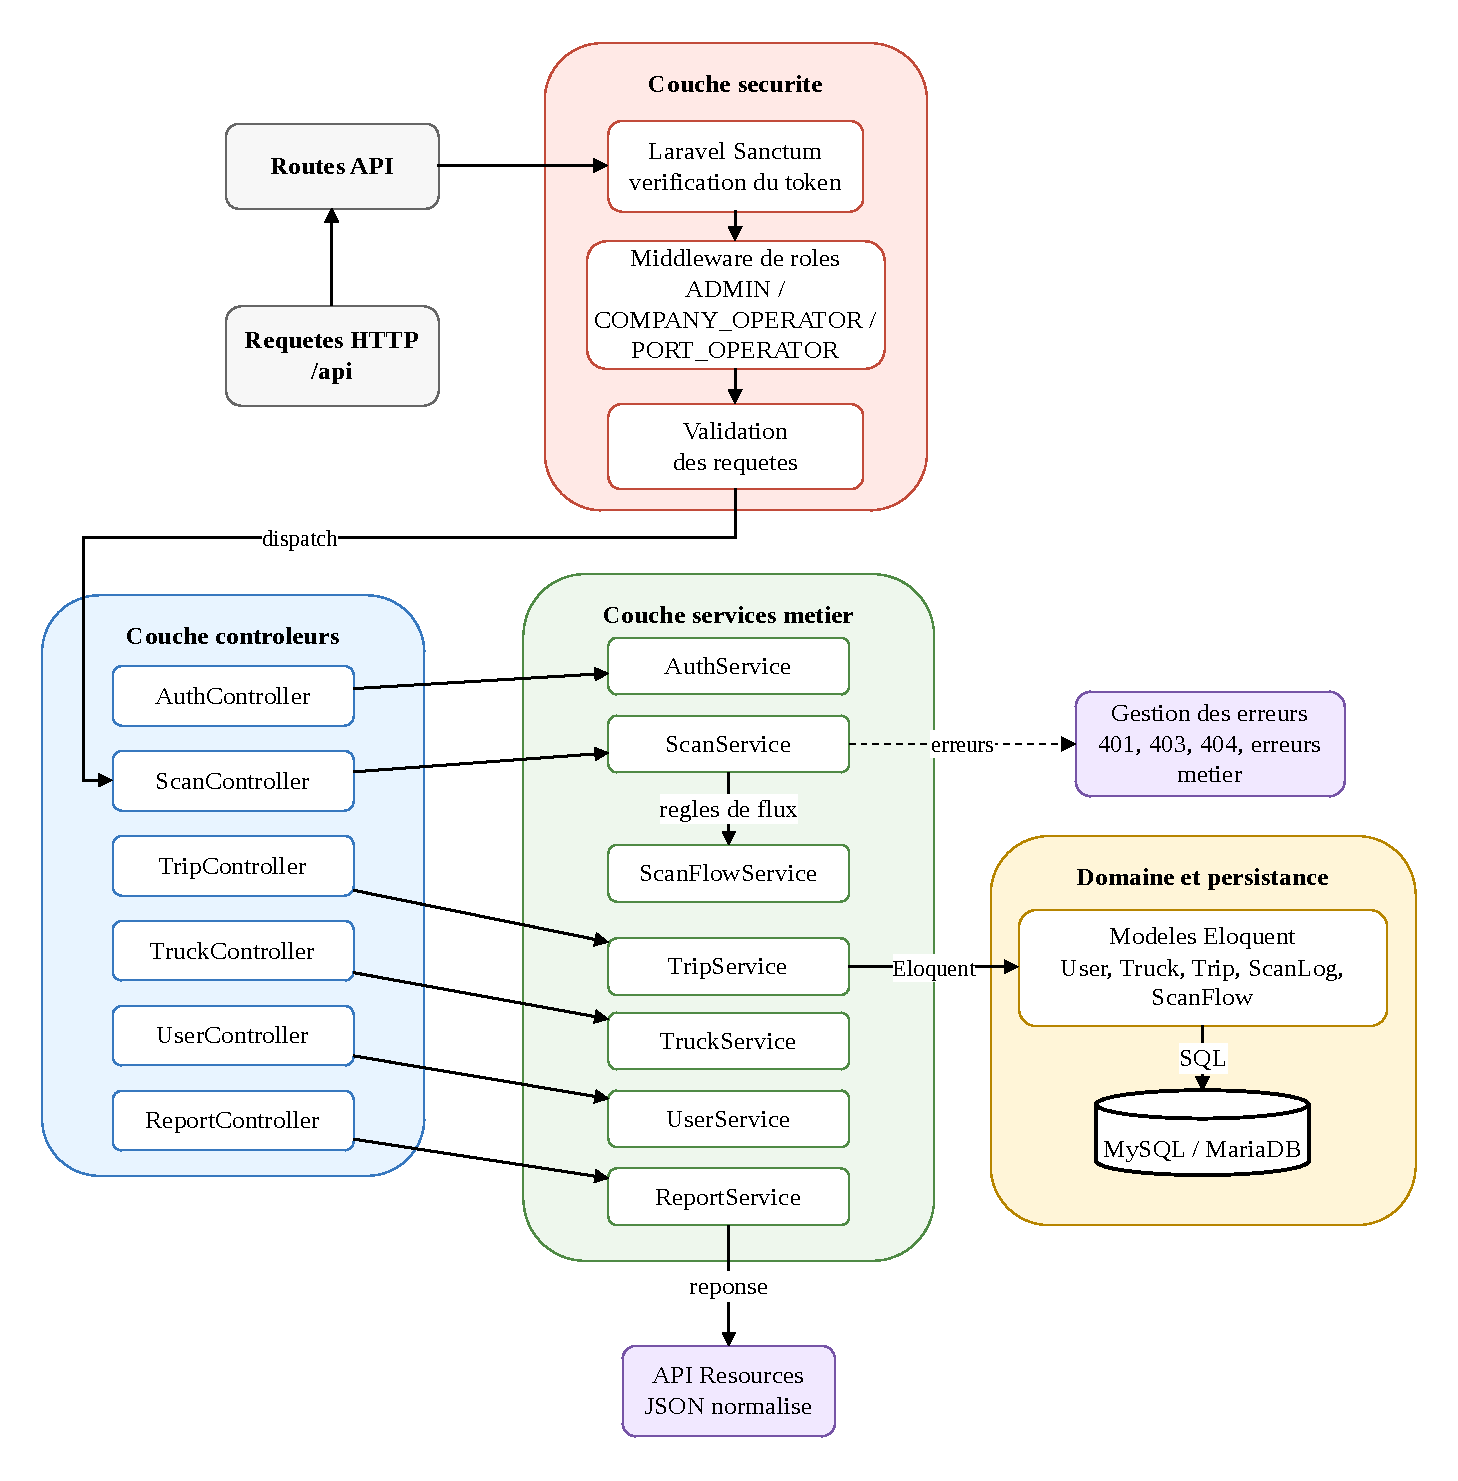
\includegraphics[width=\textwidth,height=0.72\textheight,keepaspectratio]
    {figures/architecture/architecture-backend-laravel.pdf}

    \caption{Architecture interne du backend Laravel}

    \label{fig:backend-laravel-architecture}
\end{figure}

\subsection{Architecture de l'application mobile Flutter}

L'application mobile est conçue pour les opérateurs usine et port. Elle doit rester simple, rapide et adaptée à une utilisation terrain. Son rôle principal est de permettre l'authentification de l'opérateur, la lecture du QR code d'un camion, l'envoi du scan au backend et l'affichage du résultat retourné par l'API.

L'application Flutter suit une architecture orientée fonctionnalités. Les parties principales sont organisées autour des modules d'authentification, de tableau de bord opérateur et de scan. Cette organisation facilite l'évolution de l'application, car chaque fonctionnalité regroupe ses écrans, sa logique d'état et ses services associés.

La gestion d'état repose sur Riverpod. Les appels réseau sont réalisés avec Dio, tandis que le jeton d'authentification est conservé dans un stockage sécurisé. Le routage est assuré par GoRouter, avec un mécanisme de contrôle de session permettant d'afficher l'écran de connexion ou les écrans opérateur selon l'état d'authentification.

La figure~\ref{fig:mobile-flutter-architecture} présentera l'architecture interne de l'application mobile Flutter.

\begin{figure}[H]
    \centering
    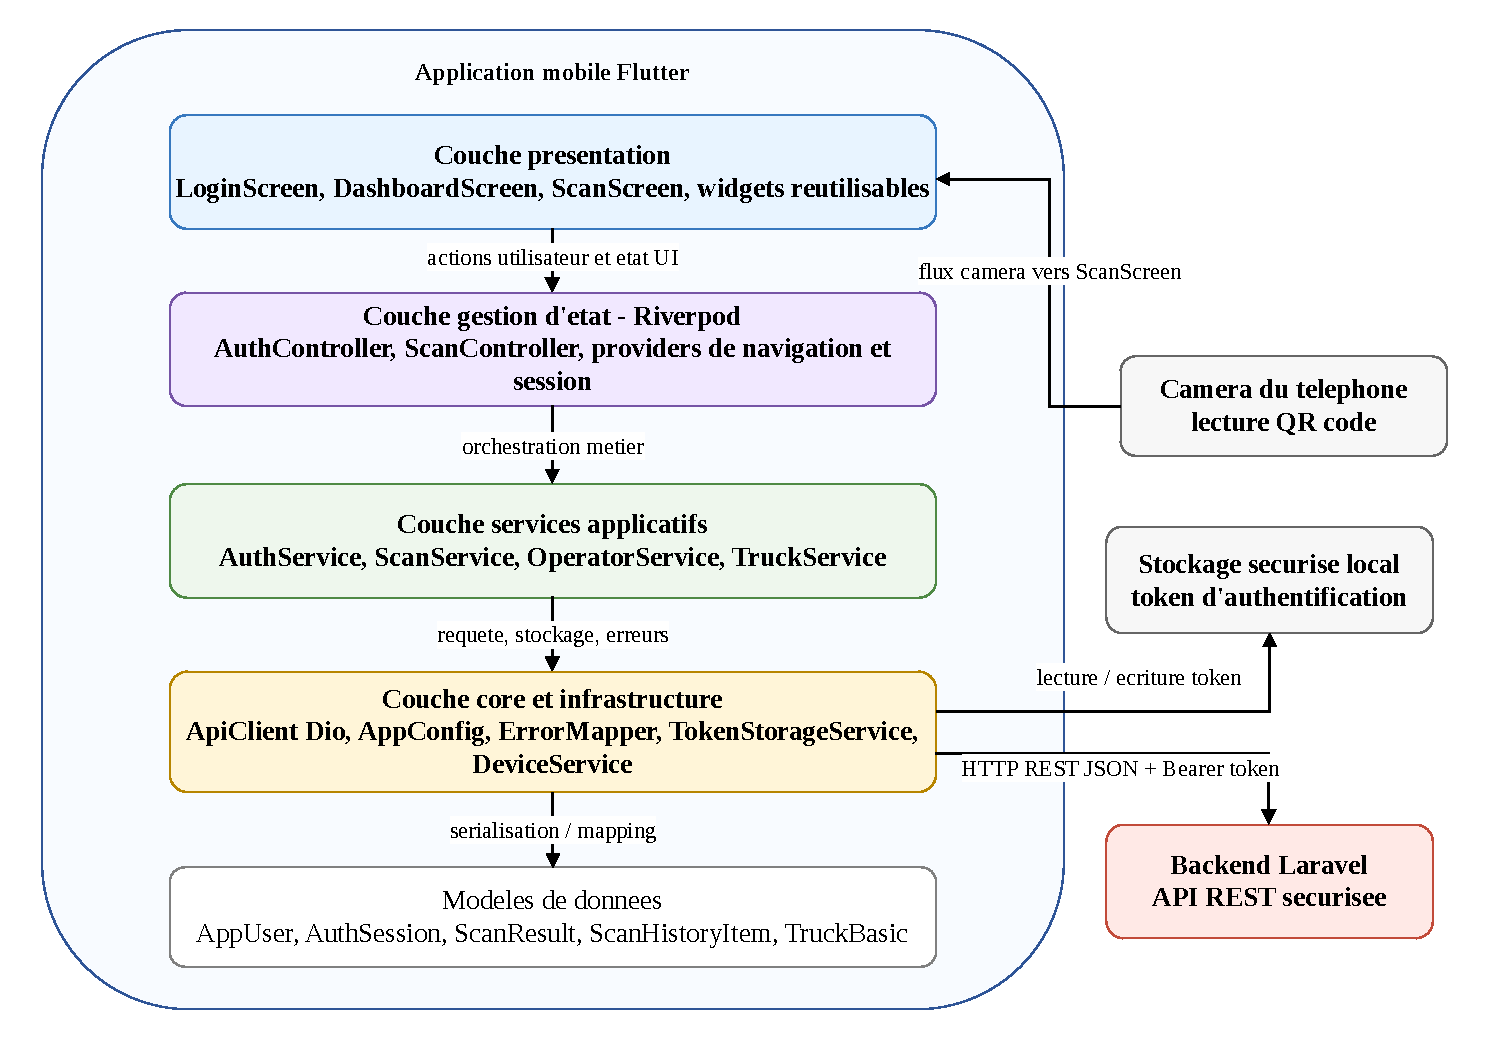
\includegraphics[width=\textwidth,keepaspectratio]
    {figures/architecture/architecture-frontend-flutter.pdf}

    \caption{Architecture interne de l'application mobile Flutter}

    \label{fig:mobile-flutter-architecture}
\end{figure}

\subsection{Architecture de l'application web React}

L'application web est une application monopage destinée à l'agent logistique. Elle fournit les interfaces de supervision et d'administration : tableau de bord, gestion des camions, gestion des utilisateurs, suivi des trajets, consultation des détails, rapports et exports.

Elle est développée avec React, TypeScript et Vite. Le routage côté client est assuré par React Router. Les routes d'administration sont protégées afin de garantir que seul un utilisateur ayant le rôle d'agent logistique puisse accéder au back-office. L'état global d'authentification est géré par Zustand, tandis qu'Axios centralise les appels vers le backend.

L'application suit une structure modulaire : les pages correspondent aux écrans principaux, les composants réutilisables assurent l'affichage des tableaux, formulaires et indicateurs, et la couche API isole la communication avec le backend. Cette séparation permet de maintenir une interface claire tout en évitant de mélanger la logique d'affichage avec la logique de communication HTTP.

La figure~\ref{fig:web-react-architecture} présentera l'architecture interne de l'application web React.

\begin{figure}[H]
    \centering
    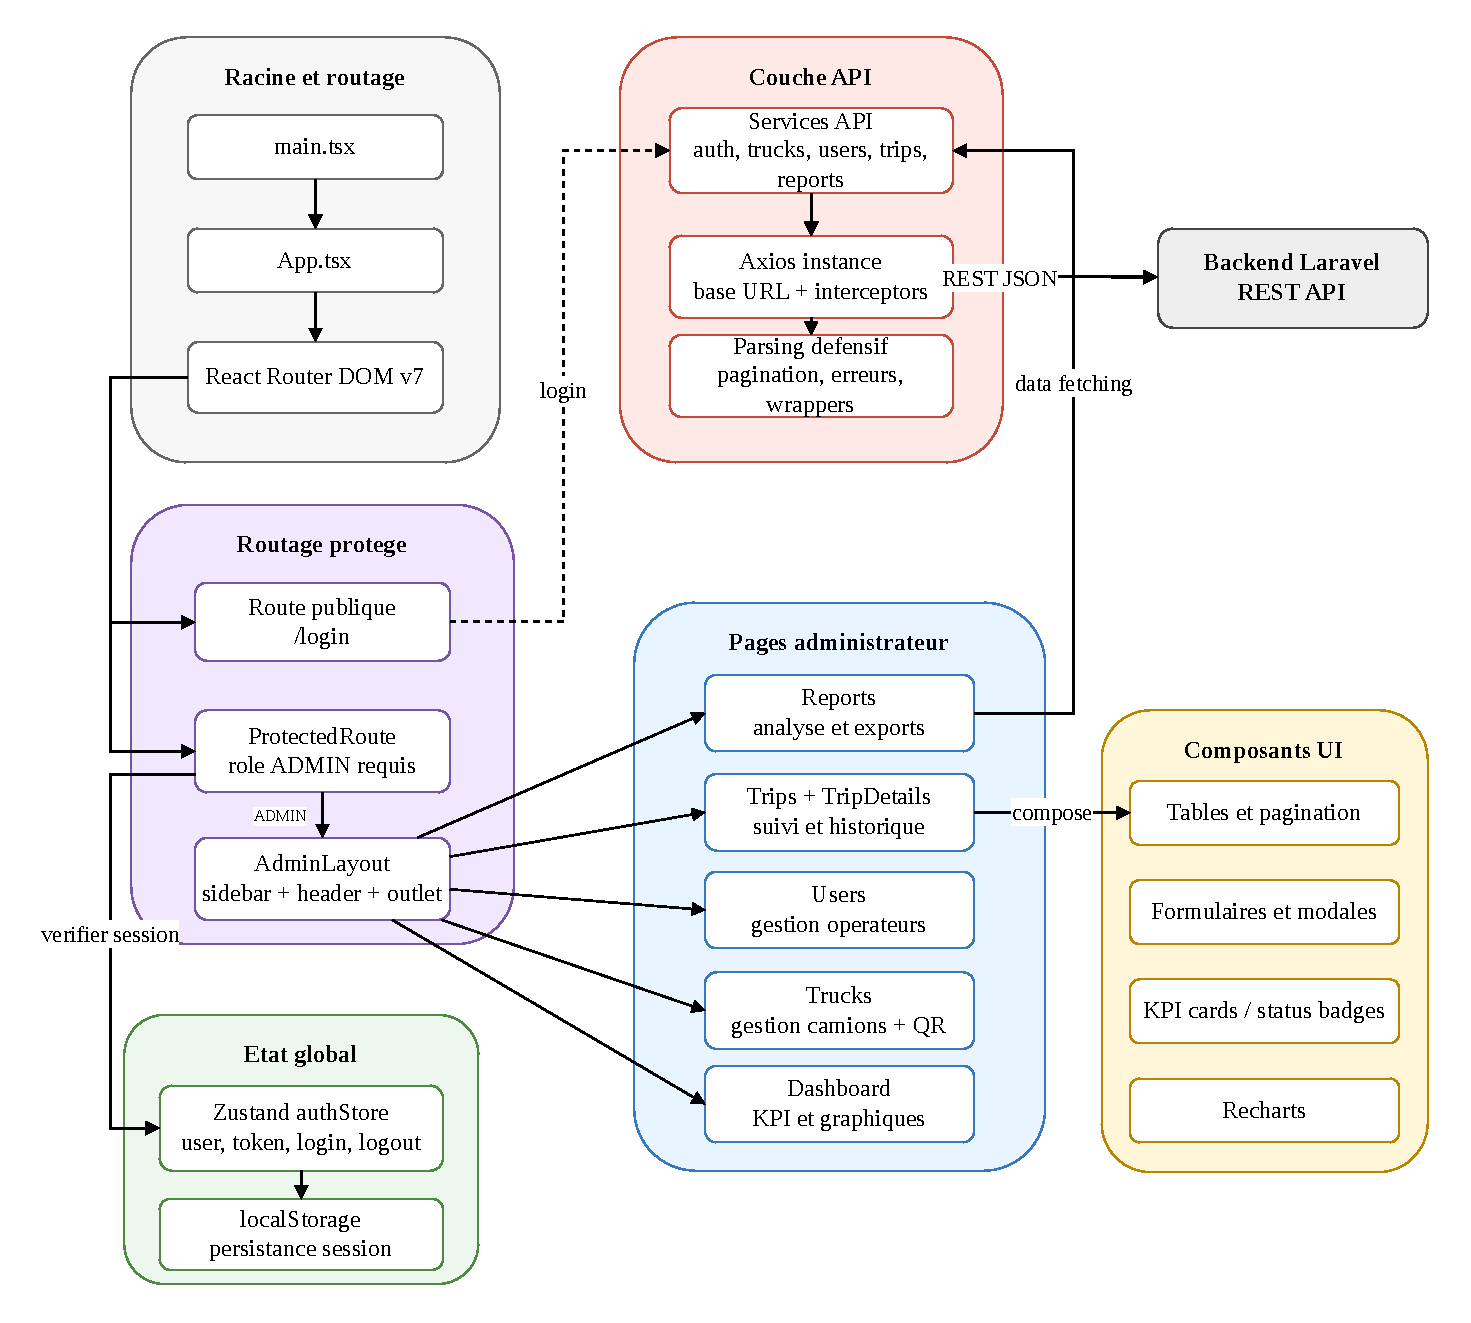
\includegraphics[width=\textwidth,height=0.72\textheight,keepaspectratio]
    {figures/architecture/architecture-frontend-react.pdf}

    \caption{Architecture interne de l'application web React}

    \label{fig:web-react-architecture}
\end{figure}

\section{Conception de la base de données et des API}

\subsection{Modèle de domaine}

Le modèle de domaine de SomaScan est centré autour du trajet. Un camion peut effectuer plusieurs trajets au cours du temps, mais il ne peut posséder qu'un seul trajet actif à un instant donné. Chaque trajet appartient à un camion et possède une séquence d'événements représentée par des logs de scan.

Un utilisateur peut effectuer plusieurs scans. Chaque log de scan est rattaché à un utilisateur, à un camion et à un trajet. Le flux de scan définit l'ordre des statuts autorisés pour le cycle de vie d'un trajet. Cette organisation permet de séparer les données de configuration du flux métier, ce qui rend le système plus adaptable en cas d'évolution du processus.

La figure~\ref{fig:diagramme-classes-domaine} présentera le diagramme de classes conceptuel du domaine.

\begin{figure}[H]
    \centering
    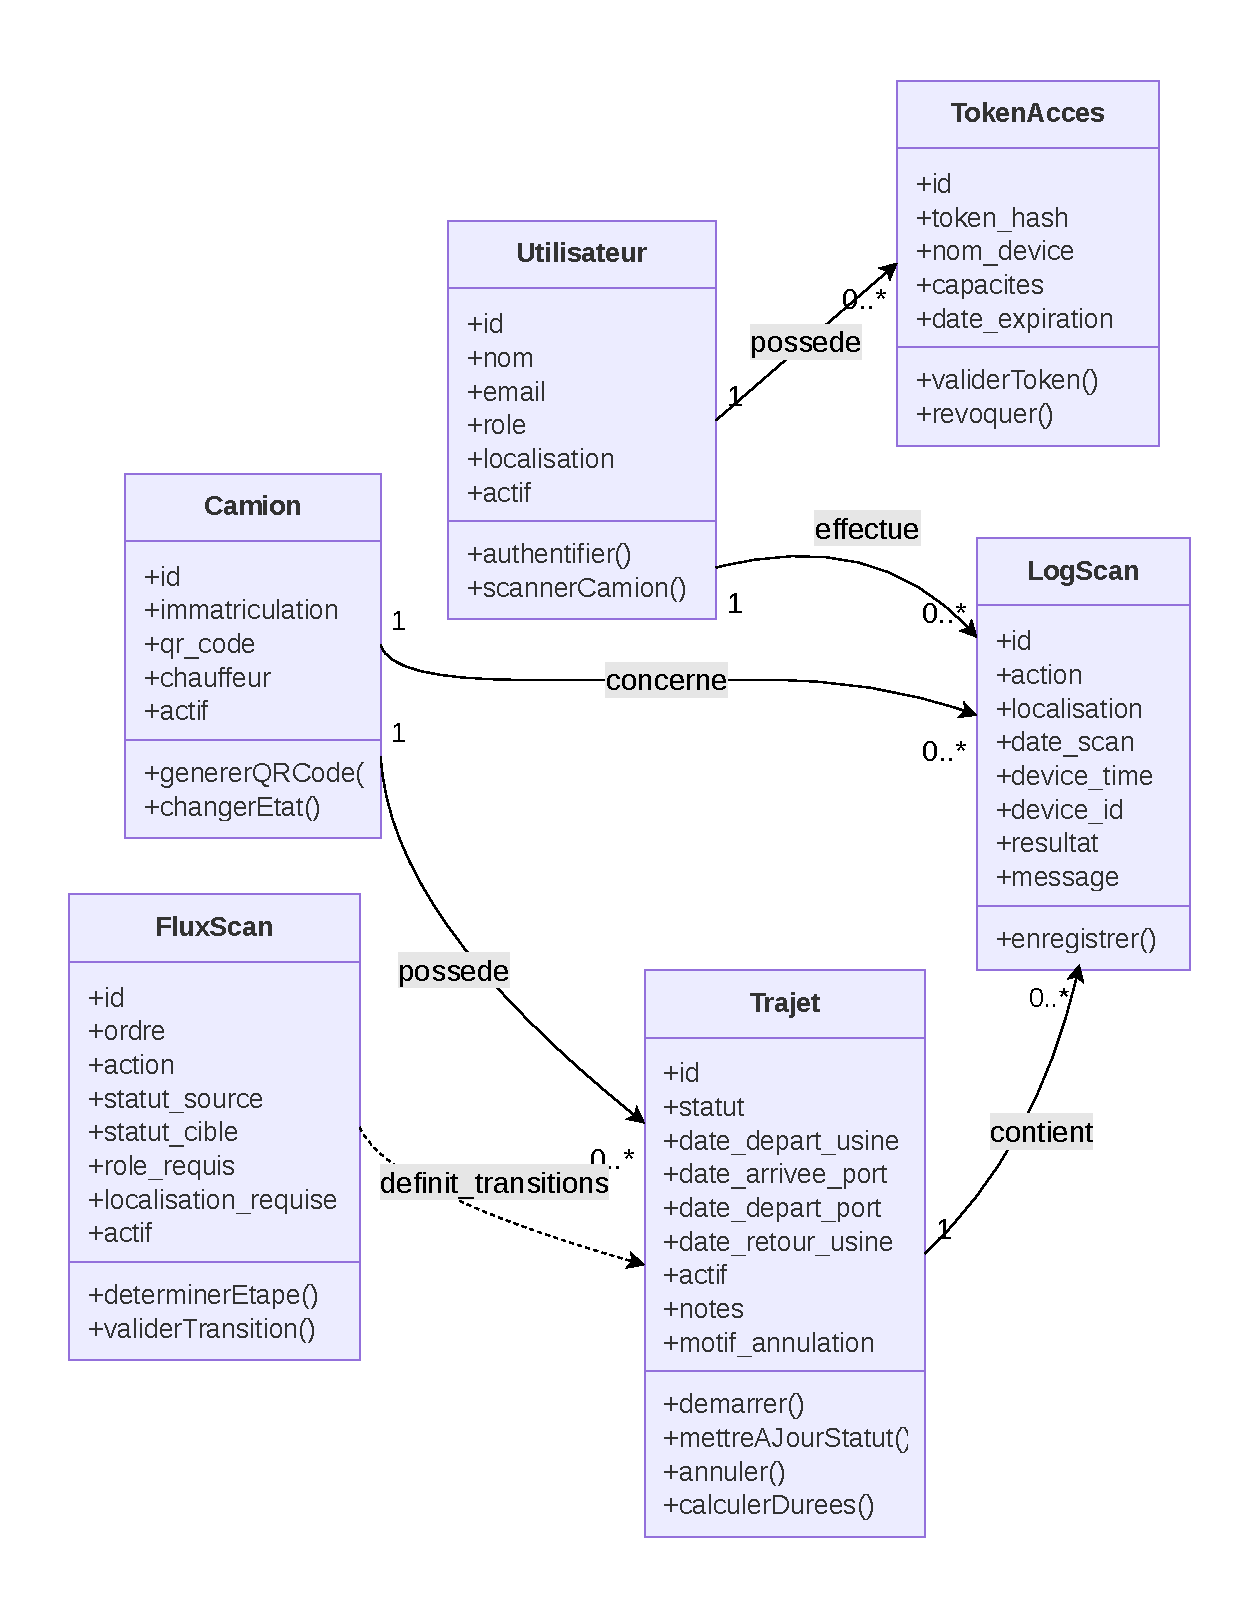
\includegraphics[width=\textwidth,keepaspectratio]
    {figures/schemas/diagramme-de-classe.pdf}

    \caption{Diagramme de classes conceptuel du domaine}

    \label{fig:diagramme-classes-domaine}
\end{figure}

\subsection{Schéma relationnel}

La base de données contient les tables métier principales suivantes : \path{users}, \path{trucks}, \path{trips}, \path{scan_logs} et \path{scan_flows}. La table \path{users} stocke les profils et les rôles. La table \path{trucks} stocke les camions, leurs immatriculations, leurs chauffeurs, leurs QR codes et leur état actif. La table \path{trips} représente les trajets avec leurs statuts et leurs dates de passage. La table \path{scan_logs} conserve l'historique détaillé des scans. La table \path{scan_flows} stocke la séquence active des statuts du flux de scan.

Des tables techniques sont également utilisées par Laravel, notamment pour les jetons d'accès Sanctum, les sessions, le cache et les files de jobs. Ces tables ne constituent pas le coeur métier de SomaScan, mais elles participent au fonctionnement de l'application.

Plusieurs contraintes garantissent l'intégrité des données. Le numéro d'immatriculation et le QR code d'un camion sont uniques. Un index unique permet d'empêcher qu'un camion possède plusieurs trajets actifs en même temps. Les clés étrangères relient les trajets aux camions, les logs aux trajets, aux camions et aux utilisateurs. Les suppressions en cascade permettent de maintenir la cohérence lorsque certaines données sont supprimées.

La figure~\ref{fig:schema-relationnel-db} présentera le schéma relationnel de la base de données.

\begin{figure}[H]
    \centering
    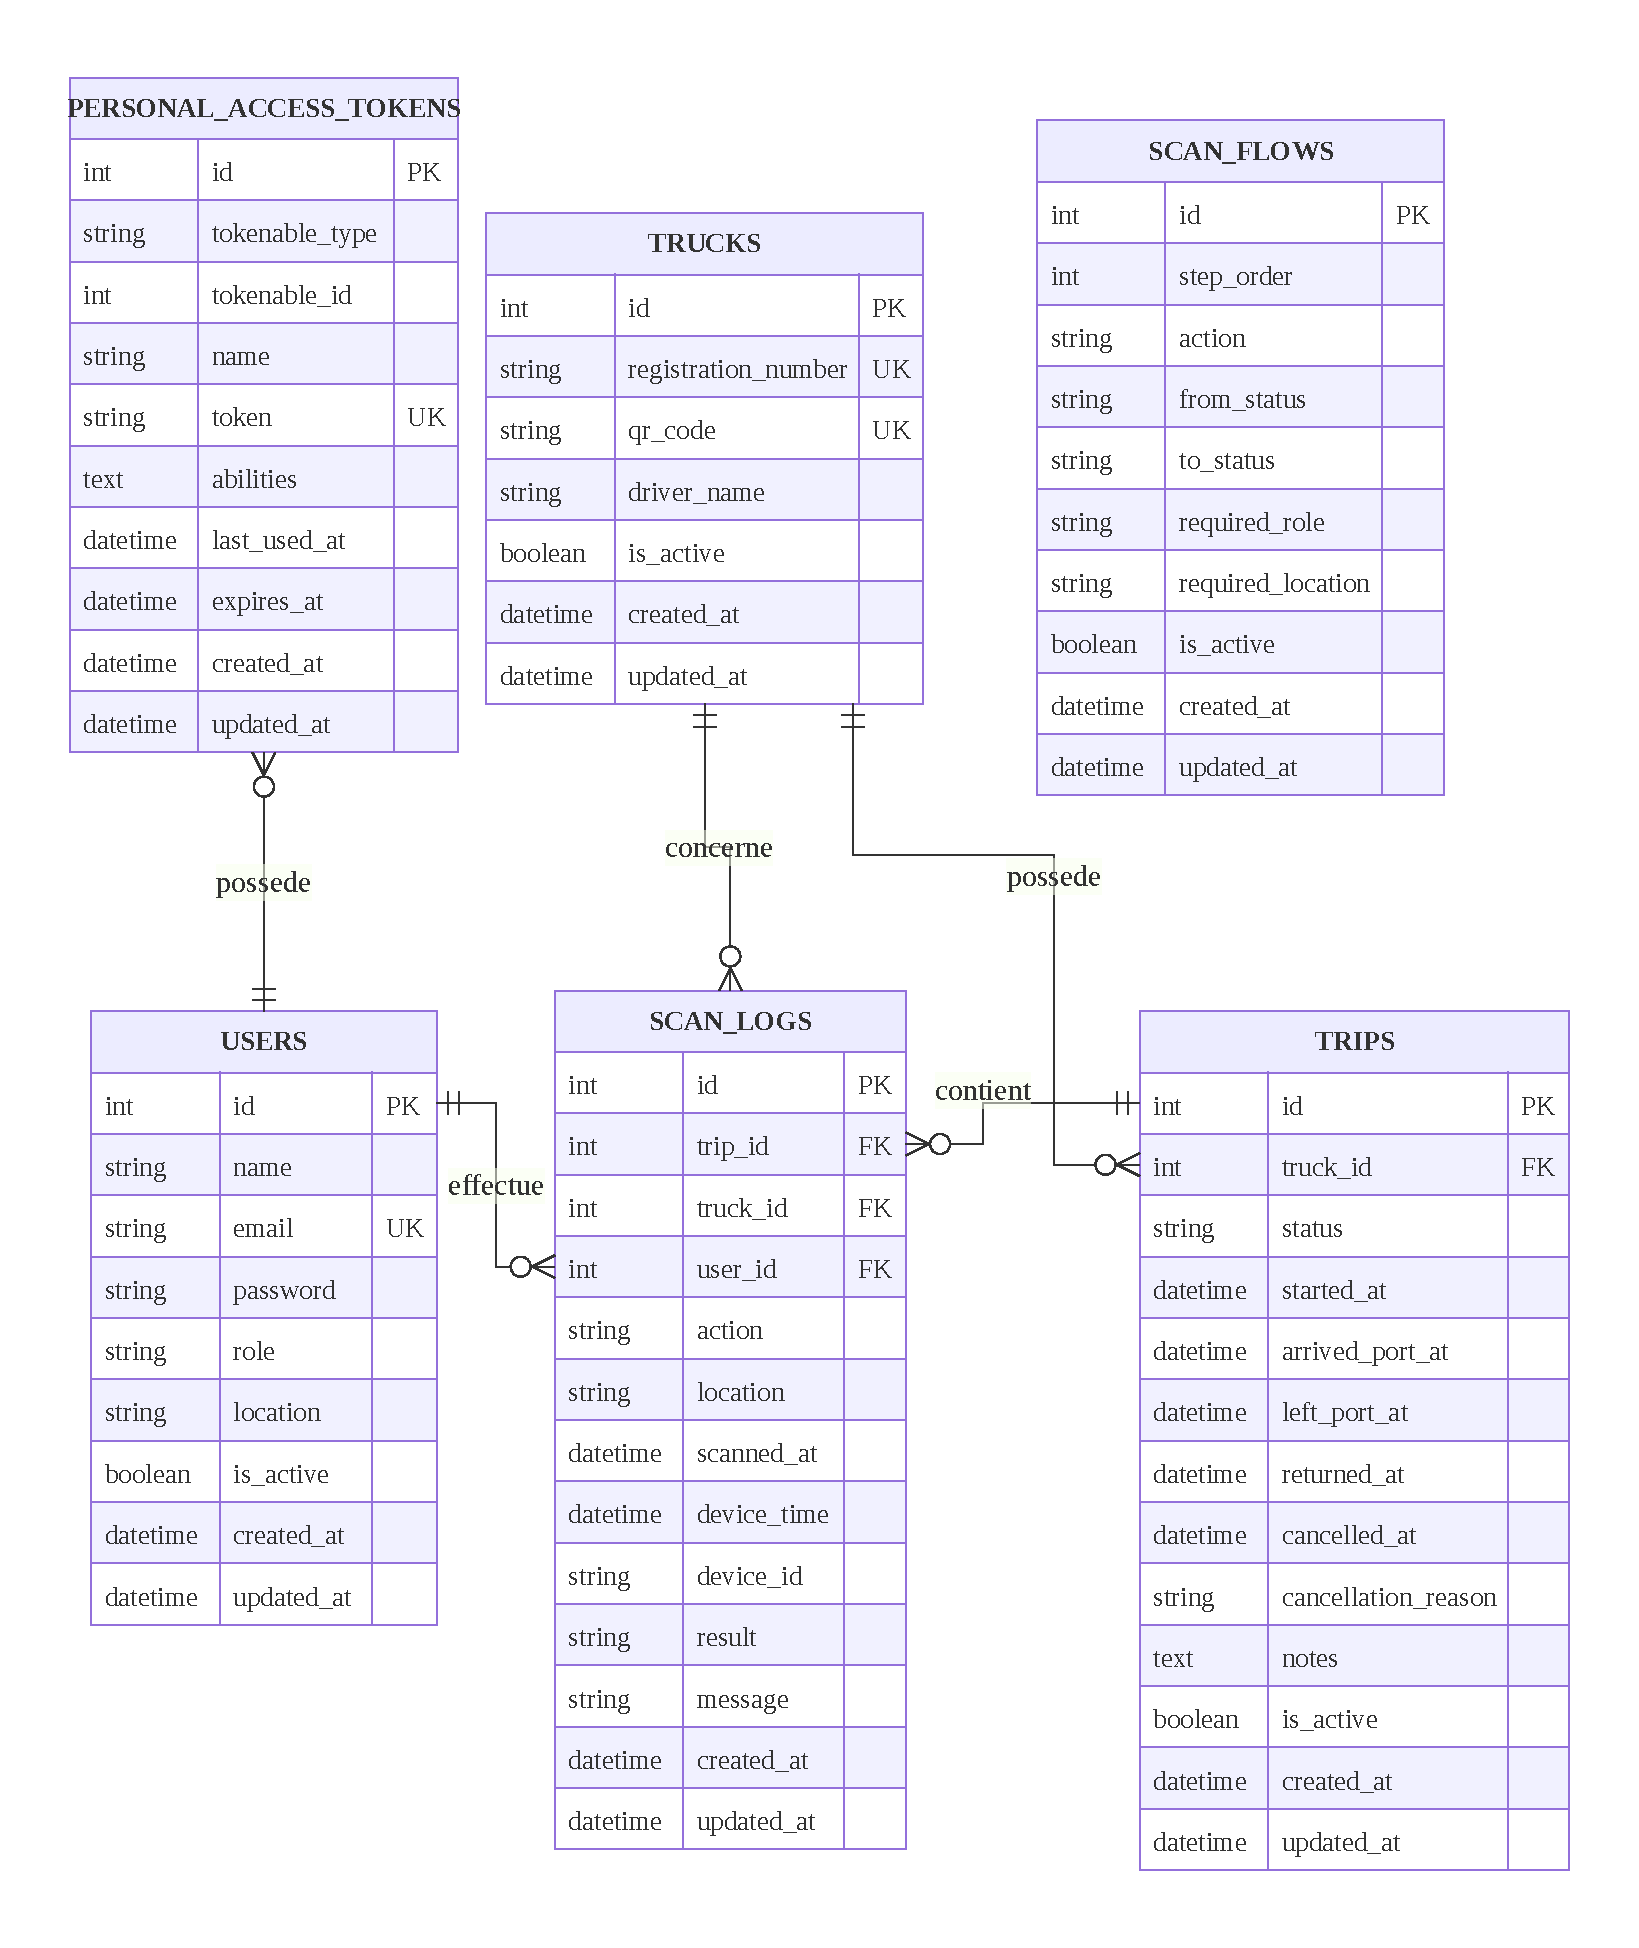
\includegraphics[width=\textwidth,keepaspectratio]
    {figures/schemas/schema-relationel-db.pdf}

    \caption{Schéma relationnel de la base de données}

    \label{fig:schema-relationnel-db}
\end{figure}

\subsection{Organisation des API REST}

Le backend expose une API REST préfixée par \texttt{/api}. Les réponses suivent une structure JSON standardisée comprenant un indicateur de succès, les données retournées, un message et éventuellement des erreurs de validation. Cette normalisation facilite l'intégration avec les applications Flutter et React.

Les endpoints sont regroupés par domaine fonctionnel : authentification, scan, camions, trajets, utilisateurs, dashboard, logs, rapports et configuration du flux de scan. Les opérateurs utilisent principalement les endpoints d'authentification, de scan, d'historique récent et d'information basique du camion. L'agent logistique utilise les endpoints d'administration pour la gestion complète et le suivi analytique.

La figure~\ref{fig:schema-api-rest} présentera l'organisation des API REST principales par module.

\begin{figure}[H]
    \centering
    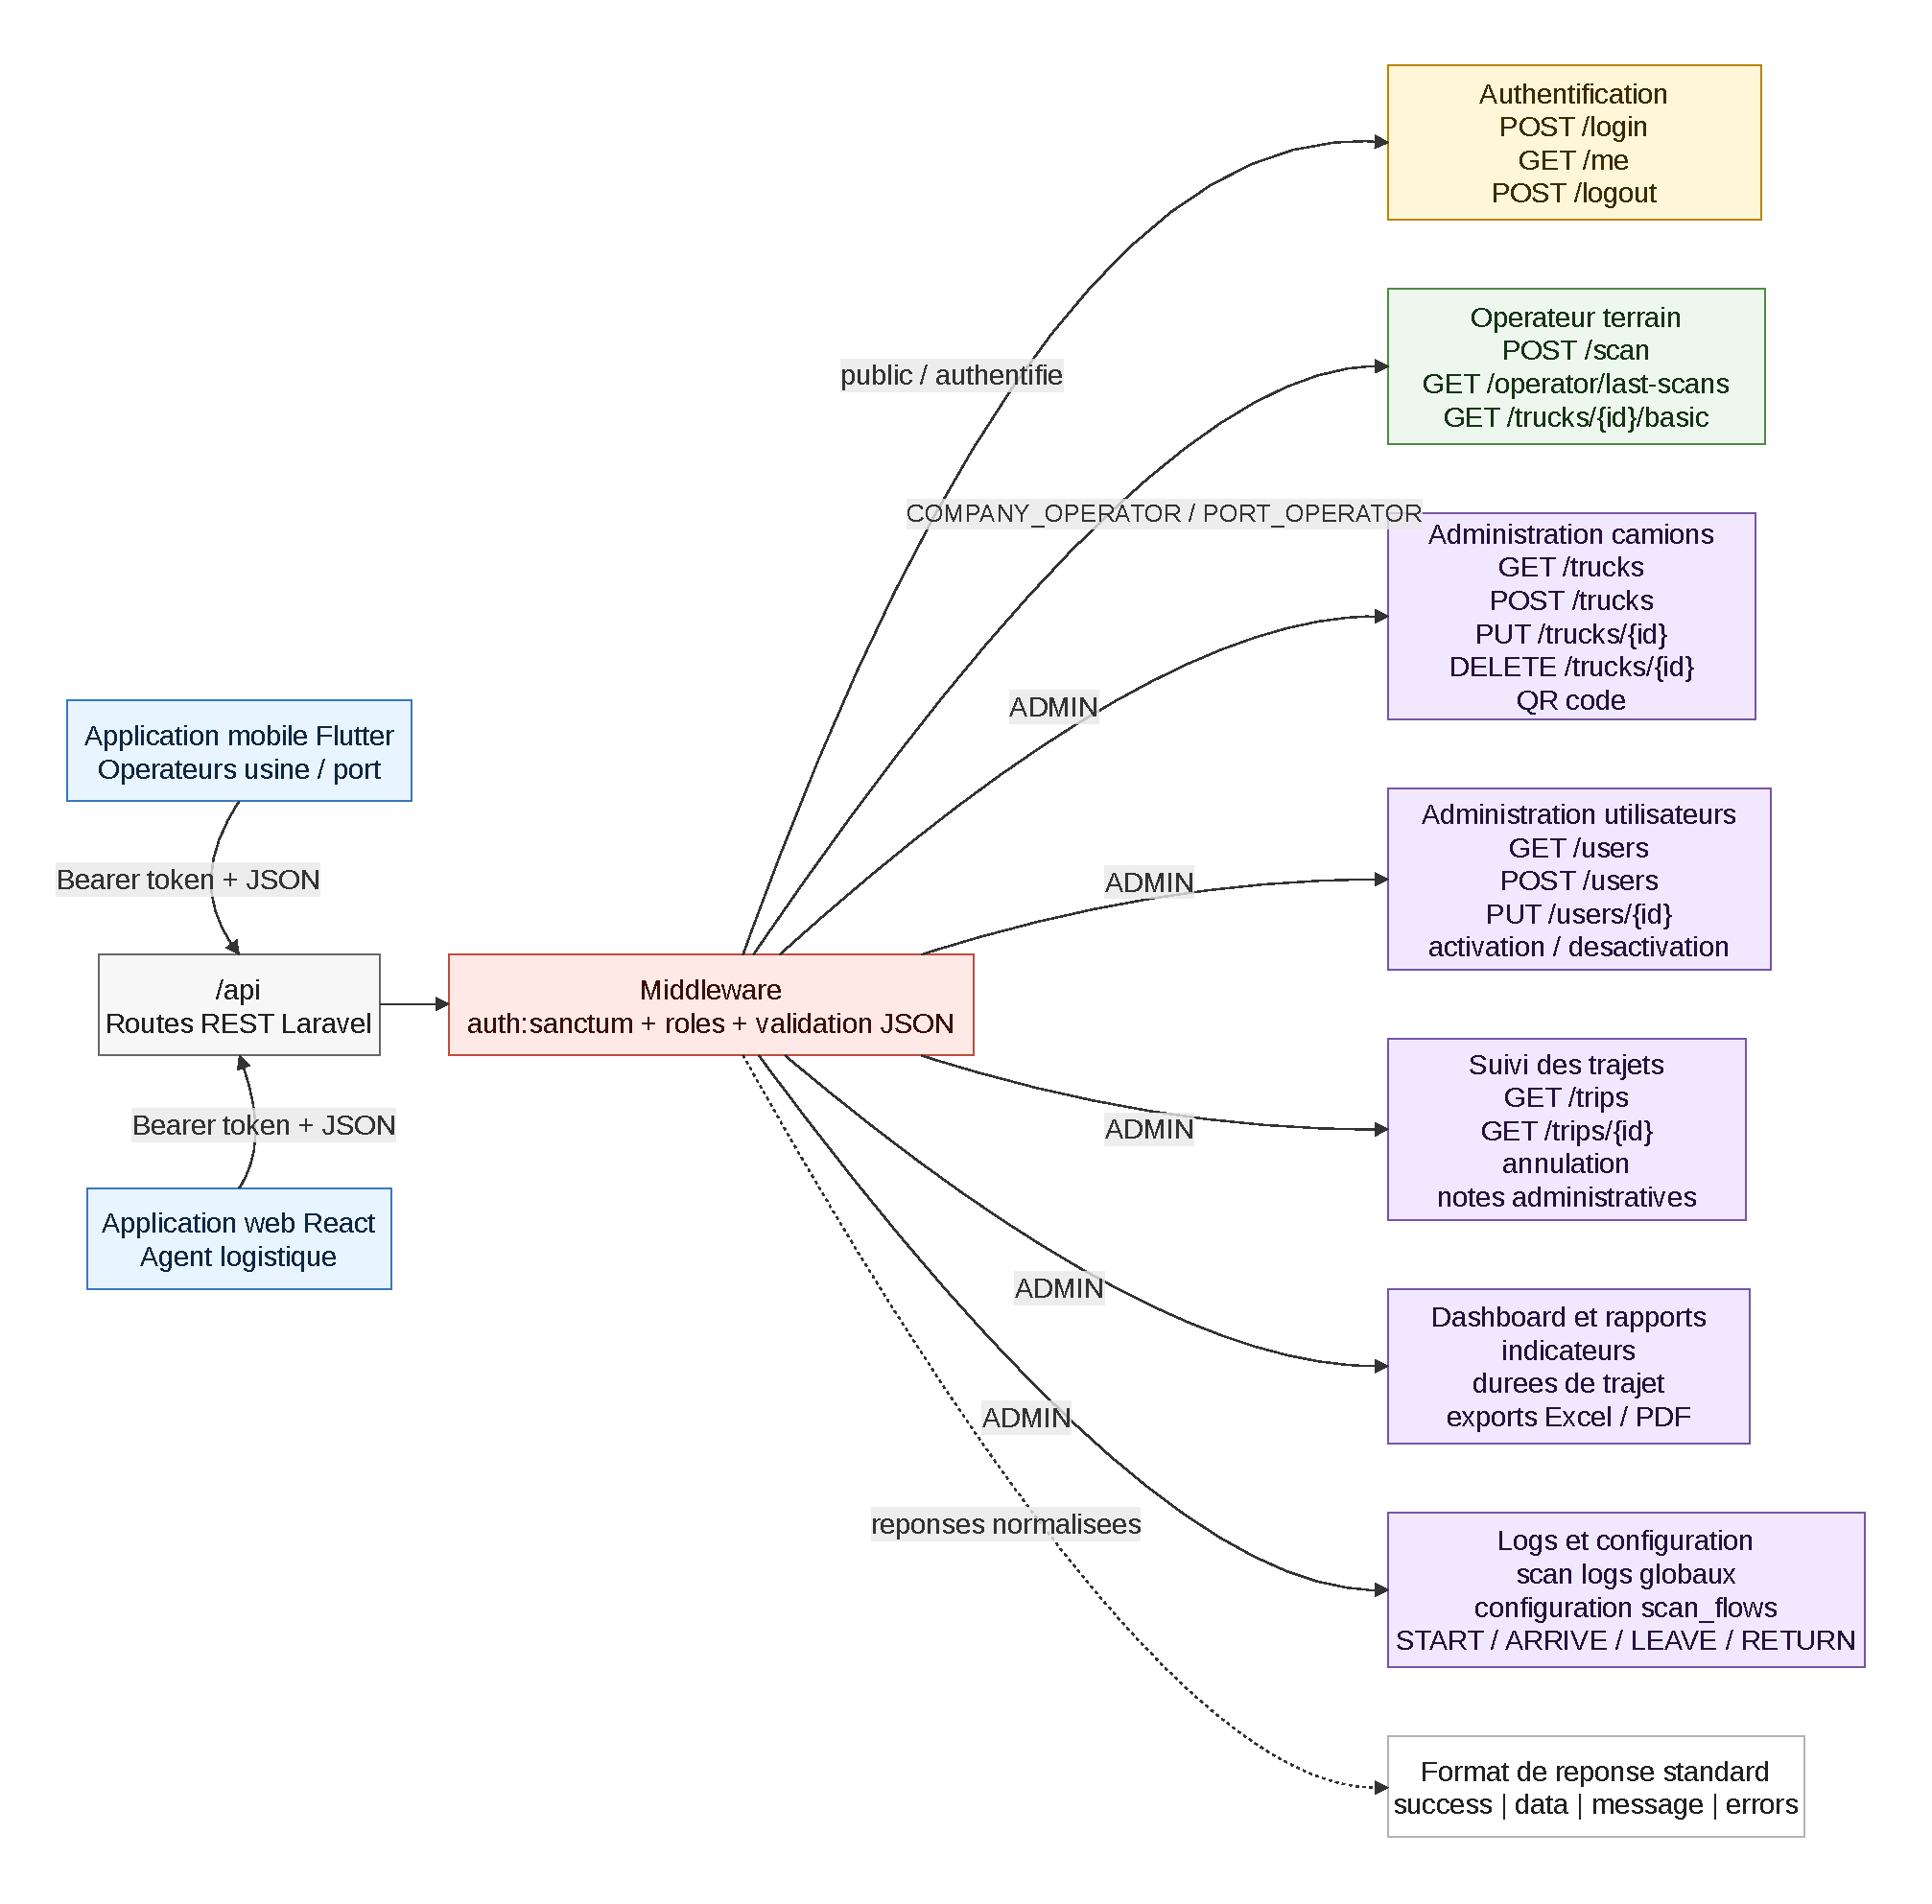
\includegraphics[width=\textwidth,keepaspectratio]
    {figures/schemas/schema-api.pdf}

    \caption{Organisation des API REST principales par module}

    \label{fig:schema-api-rest}
\end{figure}

\subsection{Séquence de scan QR}

Le scénario de scan QR est le processus métier le plus critique du système. Lorsqu'un opérateur scanne un camion, l'application mobile envoie le contenu du QR code au backend. Le backend résout le camion concerné, vérifie qu'il est actif, détermine le trajet courant et calcule l'action attendue selon le flux de scan configuré.

Le système vérifie ensuite que le rôle et la localisation de l'opérateur correspondent à l'action demandée. Si l'opération est valide, le trajet est créé ou mis à jour, un log de scan est enregistré et une réponse est retournée à l'application mobile avec le statut courant et l'étape suivante. En cas d'erreur, le backend retourne un message explicite : camion introuvable, camion inactif, rôle non autorisé, trajet déjà terminé ou flux non configuré.

La figure~\ref{fig:sequence-scan-qr-statut} présentera le diagramme de séquence du scan QR et de la mise à jour du statut.

\begin{figure}[H]
    \centering
    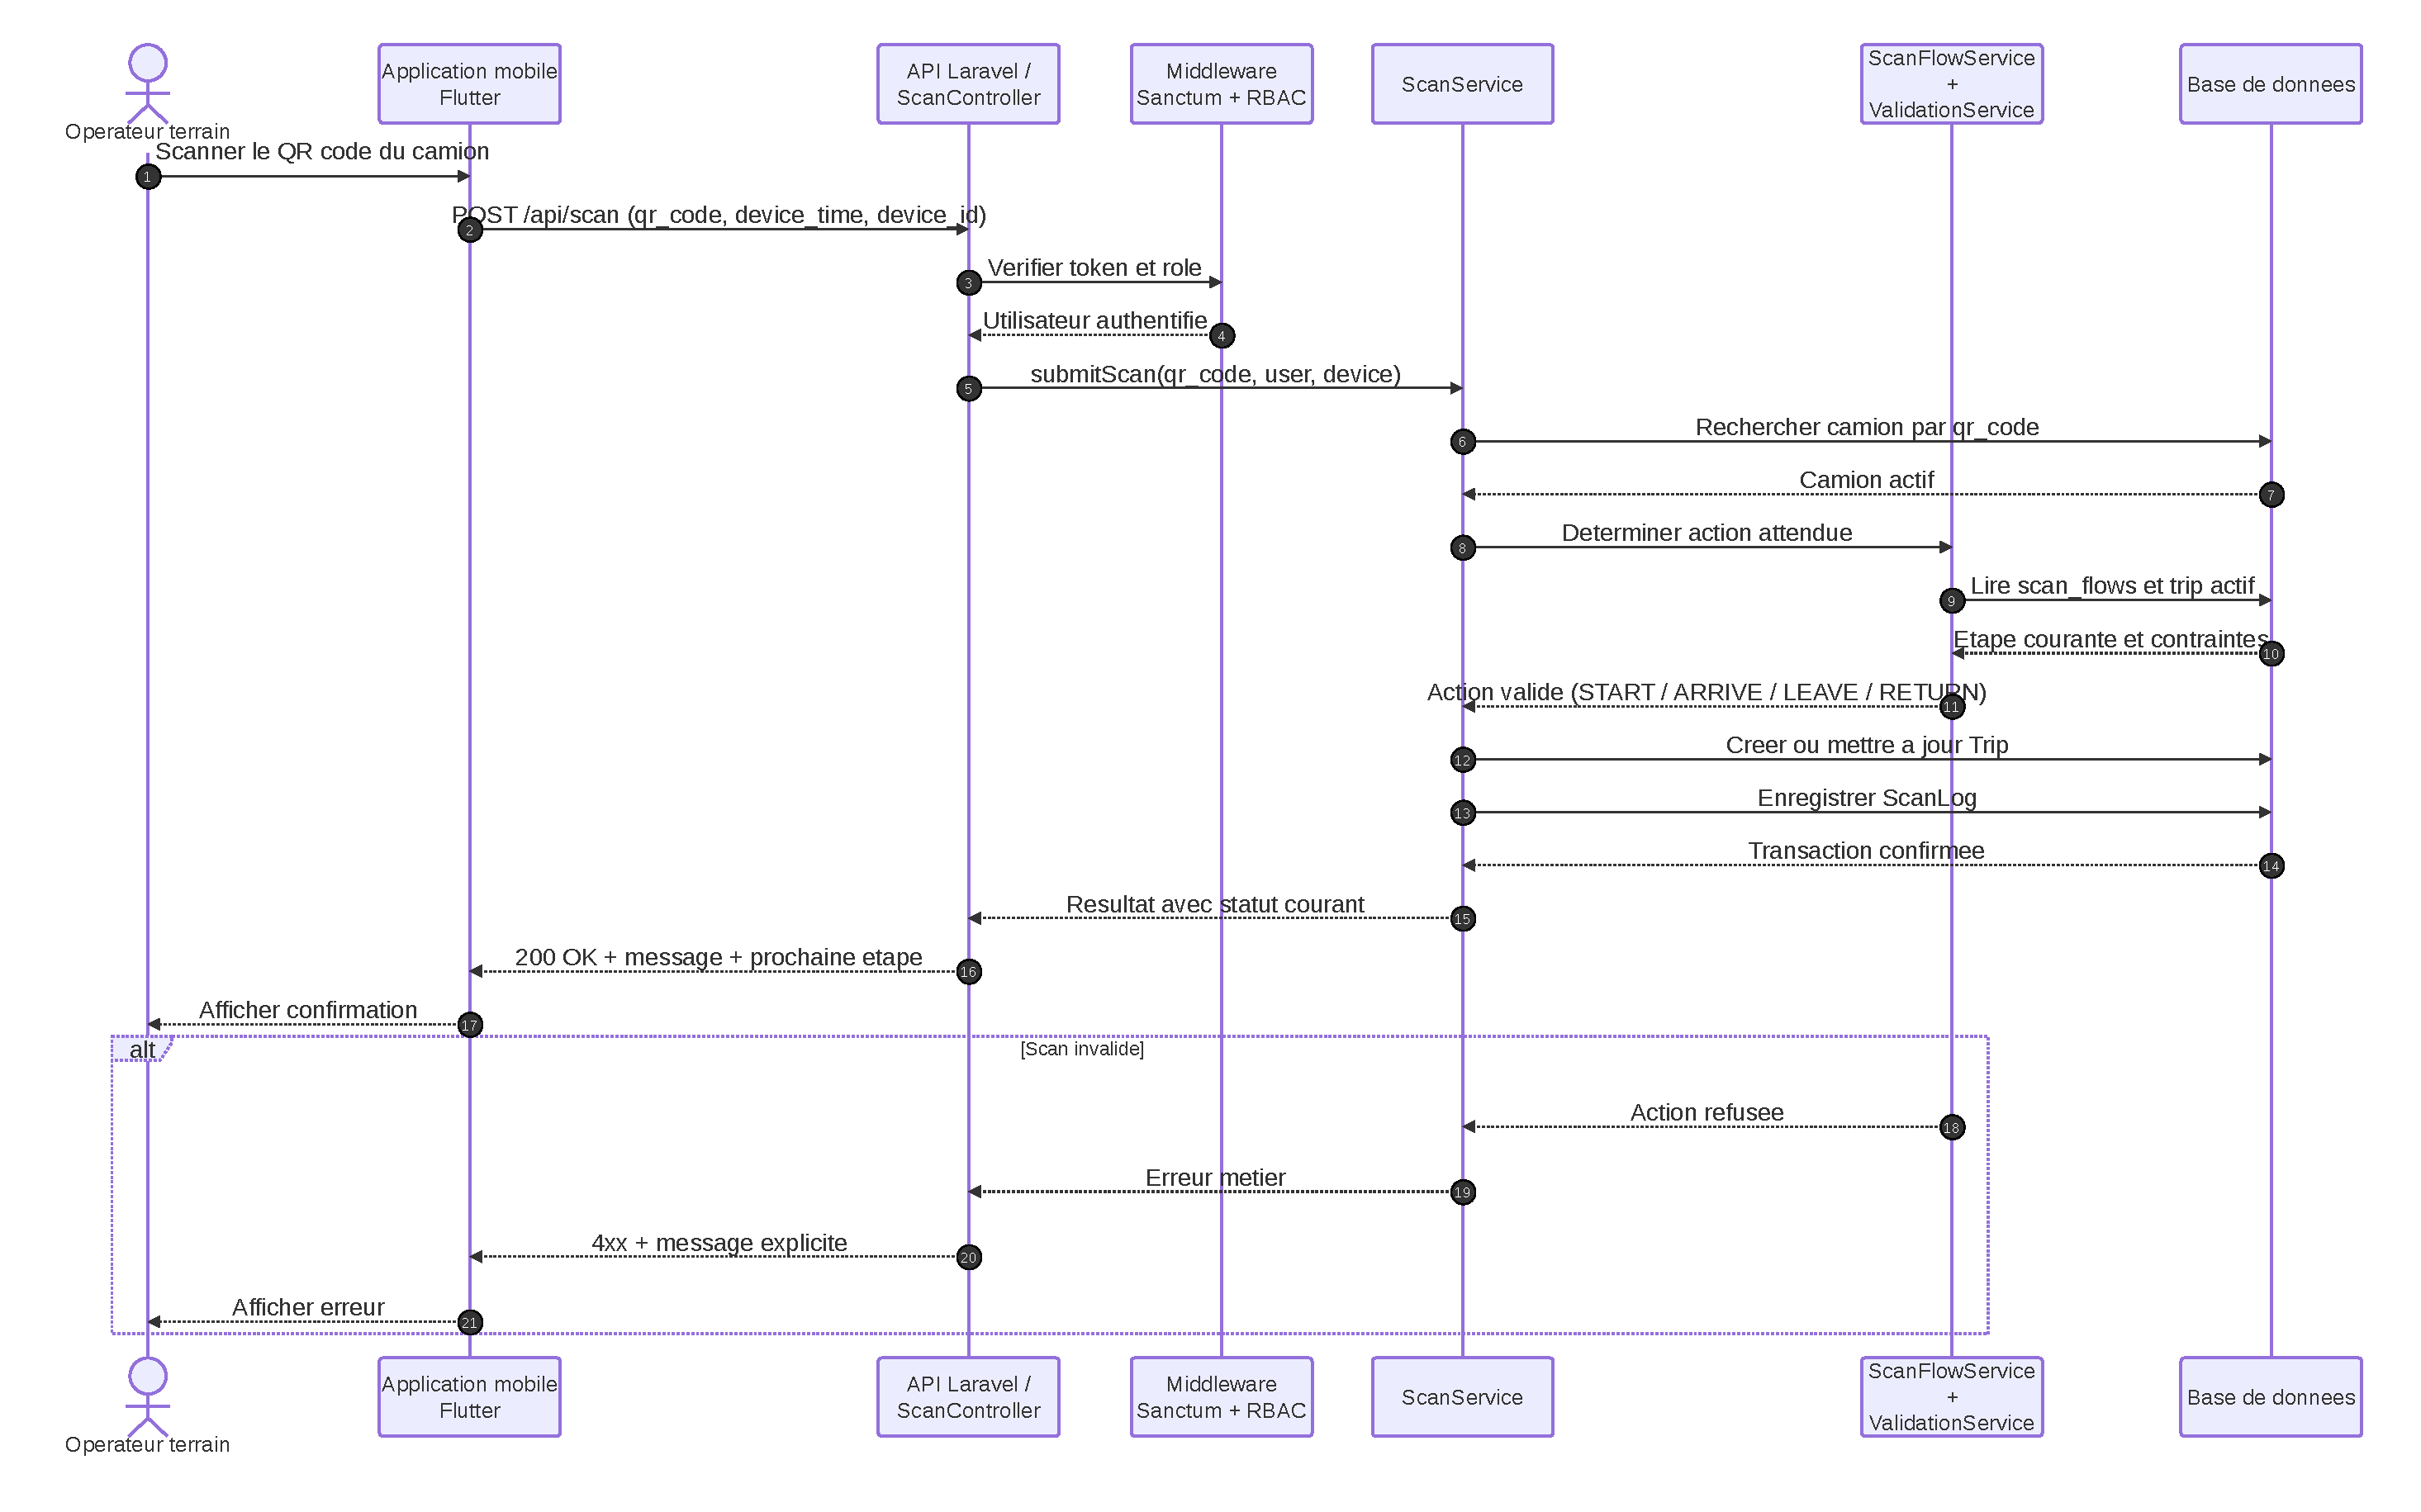
\includegraphics[width=\textwidth,height=0.72\textheight,keepaspectratio]
    {figures/diagrams/diagramme-sequence-scanQR.pdf}

    \caption{Séquence de scan QR et mise à jour du statut}

    \label{fig:sequence-scan-qr-statut}
\end{figure}

\section{Conception de la sécurité}

La sécurité de SomaScan repose sur plusieurs niveaux complémentaires. Le premier niveau est l'authentification par jeton, assurée par Laravel Sanctum. Après connexion, l'utilisateur reçoit un jeton d'accès utilisé par les applications clientes pour appeler les endpoints protégés.

Le second niveau est le contrôle des rôles. Chaque utilisateur possède un rôle : agent logistique, opérateur usine ou opérateur port. Les routes sensibles sont protégées par middleware afin de limiter l'accès aux fonctionnalités autorisées. L'application web vérifie également que l'utilisateur connecté possède le rôle d'agent logistique avant d'afficher les pages d'administration.

Le troisième niveau concerne la validation métier des scans. Même si un utilisateur est authentifié, il ne peut effectuer que les actions compatibles avec son rôle et sa localisation. Ainsi, un opérateur port ne peut pas démarrer ou clôturer un trajet, tandis qu'un opérateur usine ne peut pas enregistrer l'arrivée ou le départ du port.

La figure~\ref{fig:sequence-authentification-roles} présentera la séquence d'authentification et de contrôle des rôles.

\begin{figure}[H]
    \centering
    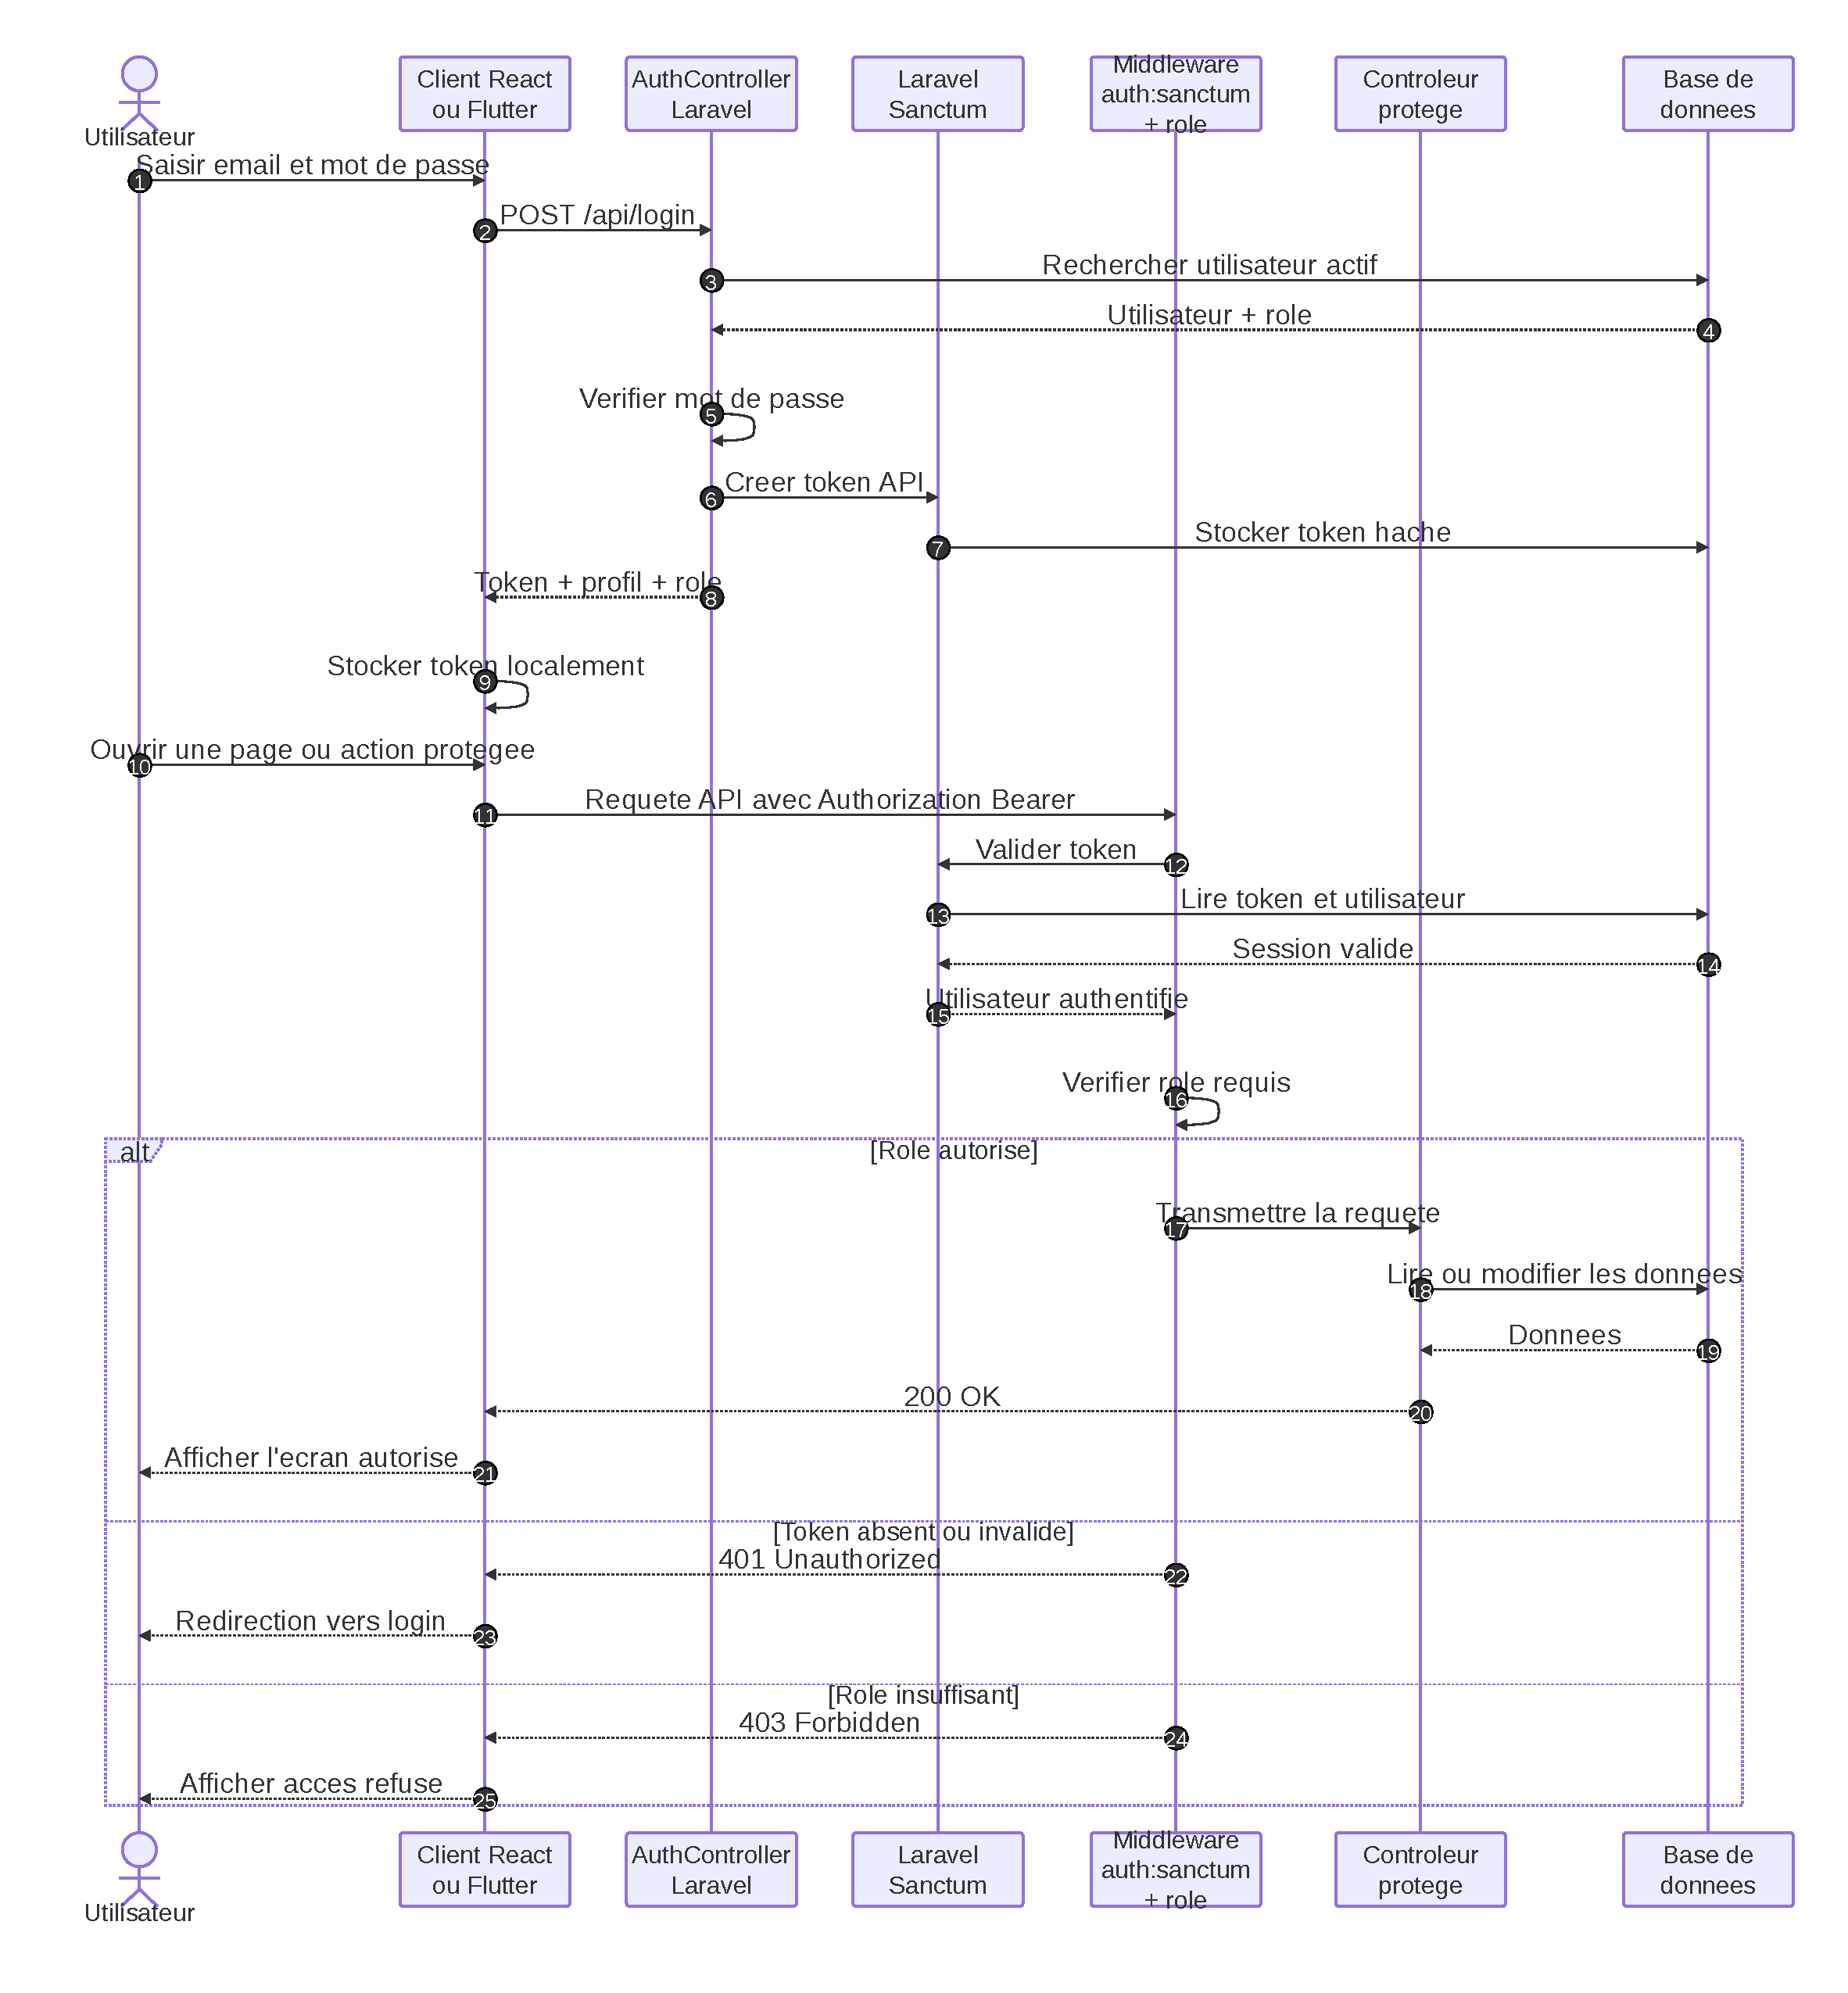
\includegraphics[width=\textwidth,height=0.72\textheight,keepaspectratio]
    {figures/diagrams/diagramme-sequence-authentification.pdf}

    \caption{Séquence d'authentification et de contrôle des rôles}

    \label{fig:sequence-authentification-roles}
\end{figure}

\section{Conclusion}

Ce chapitre a présenté la conception générale de SomaScan. L'architecture retenue sépare clairement le backend Laravel, l'application mobile Flutter et l'application web React. Le backend centralise la logique métier, la sécurité et l'accès aux données, tandis que les deux applications clientes offrent des interfaces adaptées aux opérateurs terrain et à l'agent logistique.

La conception de la base de données, des API et des mécanismes de sécurité permet de répondre aux besoins identifiés dans le chapitre précédent. Les choix d'architecture assurent la traçabilité des opérations, la cohérence du cycle de vie des trajets et l'évolutivité du système. Le chapitre suivant présentera la phase d'implémentation et les principaux éléments réalisés dans chaque application.
